\subsection*{Problema 38}

\textbf{Enunciado:}
Calcular la siguiente integral indefinida utilizando
sustitución para diferenciales binomios:
\begin{align*}
I = \int x^{-2} (4 - x^4)^{-3/4} \, dx
\end{align*}

\textbf{Solución:}
Identificamos la integral como un diferencial binomio
de la forma $\int x^m (a + bx^n)^p \, dx$, donde:
\begin{align*}
m &= -2, \quad a = 4, \quad b = -1, \quad n = 4, \quad p = -\dfrac{3}{4}
\end{align*}

Verificamos la condición de integrabilidad:
\begin{align*}
\dfrac{m + 1}{n} + p &= \dfrac{-2 + 1}{4} + \left(-\dfrac{3}{4}\right) \\
&= \dfrac{-1}{4} - \dfrac{3}{4} = -1
\end{align*}

Como el resultado es un número entero, aplicamos
la sustitución sugerida:
\begin{align*}
4x^{-4} - 1 = z^4 \implies 4x^{-4} = z^4 + 1
\end{align*}

Despejamos $x^{-4}$ y luego $x$:
\begin{align*}
x^{-4} &= \dfrac{z^4 + 1}{4} \\
x &= 2(z^4 + 1)^{-1/4}
\end{align*}

Calculamos el diferencial $dx$:
\begin{align*}
dx &= -\dfrac{1}{2}(z^4 + 1)^{-5/4}(4z^3) \, dz \\
&= -2z^3 (z^4 + 1)^{-5/4} \, dz
\end{align*}

Reescribimos el término binomial en función de $z$:
\begin{align*}
4 - x^4 &= 4 - \dfrac{4}{z^4 + 1} = \dfrac{4(z^4 + 1) - 4}{z^4 + 1} \\
&= \dfrac{4z^4}{z^4 + 1}
\end{align*}

Elevamos a la potencia $-3/4$:
\begin{align*}
(4 - x^4)^{-3/4} &= \left(\dfrac{4z^4}{z^4 + 1}\right)^{-3/4} \\
&= 4^{-3/4} z^{-3} (z^4 + 1)^{3/4}
\end{align*}

Sustituimos $x^{-2}$, el binomio y $dx$ en la integral:
\begin{align*}
I &= \int \left(\dfrac{z^4+1}{4}\right)^{1/2} 
\left[4^{-3/4} z^{-3} (z^4+1)^{3/4}\right] \\
&\quad \cdot \left[-2z^3 (z^4+1)^{-5/4}\right] \, dz
\end{align*}

Simplificamos la expresión algebraica:
\begin{align*}
I &= -2 \cdot \dfrac{1}{2} \cdot \dfrac{1}{4^{3/4}} \int z^{-3} z^3 \\
&\quad \cdot (z^4+1)^{1/2 + 3/4 - 5/4} \, dz \\
&= -\dfrac{1}{4^{3/4}} \int (z^4 + 1)^{0} \, dz \\
&= -\dfrac{1}{4^{3/4}} \int 1 \, dz = -\dfrac{z}{4^{3/4}} + C
\end{align*}

Regresamos a la variable original $x$ usando
$z = (4x^{-4} - 1)^{1/4}$:
\begin{align*}
I &= -\dfrac{(4x^{-4} - 1)^{1/4}}{4^{3/4}} + C \\
&= -\left(\dfrac{4 - x^4}{4x^4}\right)^{1/4} \dfrac{1}{4^{3/4}} + C \\
&= -\dfrac{(4 - x^4)^{1/4}}{2x} + C
\end{align*}

Resultado final:
\begin{align*}
\int x^{-2} (4 - x^4)^{-3/4} \, dx = -\dfrac{(4 - x^4)^{1/4}}{2x} + C
\end{align*}

\begin{figure}[H]
	\centering
	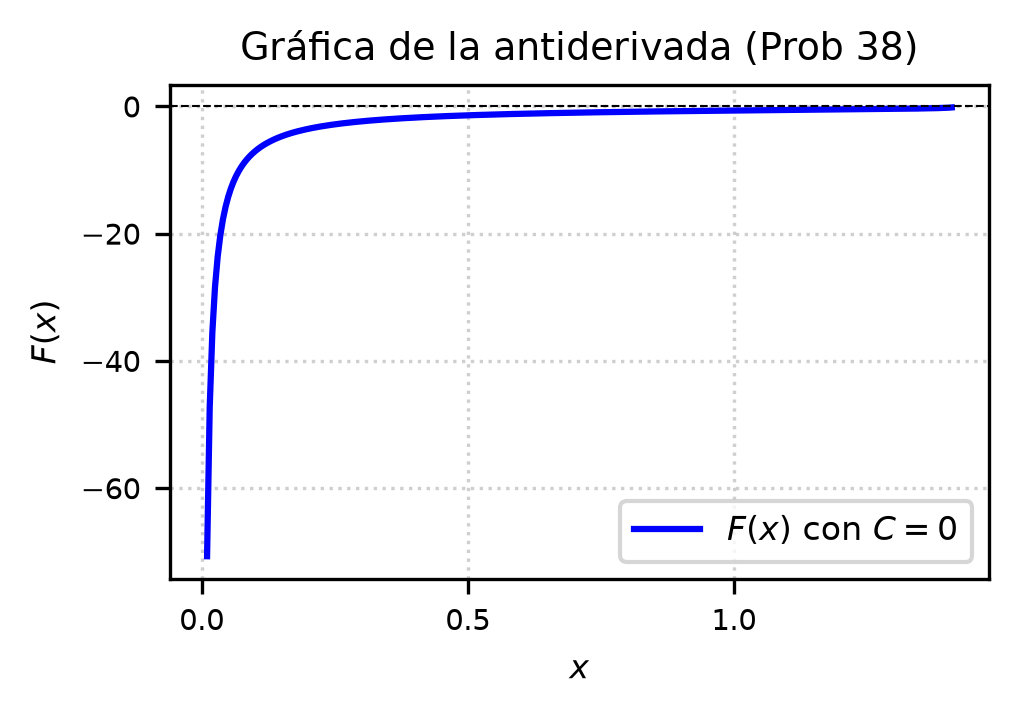
\includegraphics[width=\columnwidth]{semana_05/graficas/SEM05_P38_grafica.png}
	\caption{Representación gráfica de $f(x)$ y su antiderivada $F(x)$ evaluada para la constante de integración $C = 0$ (Problema 38).}
	\label{fig:problema38}
\end{figure}
